% Drawing 29/06-1 -- folder 29, batch 06, archive page 104 (PDF page 105).
% Transcription: au milieu de la page, à gauche, un croquis en perspective au crayon : trois diviseurs $D_{0}$, $D_{1}$, $D_{2}$ se coupant à croisements normaux, figurés par trois plans --- un plan frontal (marqué $D_{2}$ en bas à gauche), divisé en quatre par une verticale et une horizontale, d'où partent trois obliques vers un plan vertical à droite (marqué $D_{1}$), et un plan intermédiaire marqué $D_{0}$.
% Kind: three planes meeting with normal crossings (perspective sketch). Method 2 (schematic redraw from the facsimile). Status: ok.
% Notes: Pencil sketch, redrawn stroke by stroke: the front rectangle (left side, bottom in two strokes, right side, curved top) with its vertical and its horizontal middle lines; three oblique strokes rising to the right from the top, the middle and the foot of the vertical middle line; the heavy vertical stroke at the right; a faint curved stroke from the left side up to the upper left; a faint wavy stroke under the label D_0; the short faint stroke that joins the upper oblique to the top of the right vertical. Labels D_0 (upper middle), D_1 (upper right), D_2 (lower left). Still differs: it is a free perspective sketch; which stroke bounds which plane is not settled, and the strokes are drawn as they are, without being completed into three planes. The note of the transcription describes three planes whose lines of intersection meet in one point: the redraw neither confirms nor contradicts it. Overlaid 2026-11-12 (Opus 5.5) on the 400 dpi colour crop: every stroke falls on the page within one or two units; unchanged. Redrawn 2026-11-12 (issue 128): to check again. 2026-11-13, Claude Opus 5.5, overlay check (issue 147): every stroke re-read on millimetre grids of the scan rendered at 350 dpi in colour; not compiled (no TeX engine in the session), the TikZ was rasterised by a script and laid over the crop; every stroke and label now lies on its ink to within about 1 unit. Changed: the bbox was lengthened downwards (0.62 to 0.64) so that the label D_2, cut by the old crop, is whole, and D_2 moved onto it; the faint curved stroke at the left moved 2 to 3 units right onto its ink; the right side of the front rectangle is drawn as the curve it is; the bottom side runs on unbroken to a small notch after the middle vertical, then on to the right side; the lowest oblique stroke starts below the bottom side, where it crosses it; the wavy stroke under D_0 follows its ink. What still is a reading (which stroke bounds which plane) is a matter of interpretation, not of the drawing: the strokes are drawn as they are.
% Coordinates: 1 unit = 0.6 mm = 1/100 of the crop width (bbox in page fractions: [0.16, 0.43, 0.46, 0.64]).
% Redrawn by Claude (claude-fable-5-2), issue #128, 2026-11-12; not checked by a human; not compiled (no TeX in the session).
% Overlaid by Claude (claude-opus-5-5) 2026-11-12 (issue #128): rasterised from its own coordinates over the 400 dpi colour facsimile and found to match it. Not compiled. Status: partial.
% Rights: reproduces part of the work -- behind RENDER_TRANSCRIPTS, never published by itself.
\documentclass[tikz,border=3pt]{standalone}
\usepackage{amsmath,amssymb}
\usetikzlibrary{patterns,arrows.meta}
\tikzset{pencil/.style={black!45}, struck/.style={black!35}, mpt/.style={circle,draw,inner sep=1.3pt}, pt/.style={circle,fill,inner sep=0.9pt}, opt/.style={circle,draw,fill=white,inner sep=1.1pt}}
\begin{document}
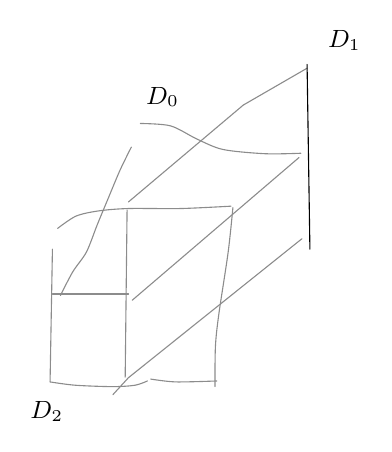
\begin{tikzpicture}[x=0.6mm,y=0.6mm,line cap=round,line join=round,font=\scriptsize]
% the front rectangle: left side, bottom, right side, curved top, middle vertical and middle horizontal
\draw[pencil] (17.2,-57.2) -- (16.7,-85.3);
\draw[pencil] plot[smooth] coordinates {(16.7,-85.3) (22,-86) (30,-86.3) (34.7,-86) (37.3,-85.1)};
\draw[pencil] plot[smooth] coordinates {(38,-84.7) (43.3,-85.3) (52,-85.1)};
\draw[pencil] plot[smooth] coordinates {(55.4,-48.4) (54.4,-57.8) (52.4,-71.1) (51.7,-77.8) (51.6,-86.3)};
\draw[pencil] plot[smooth] coordinates {(18.3,-52.8) (22.2,-50.2) (27,-49.1) (33.3,-48.6) (44.4,-48.6) (55,-48.1)};
\draw[pencil] (33,-48.9) -- (32.6,-84.3);
\draw[pencil] (17.2,-66.7) -- (33.3,-66.7);
% three oblique strokes rising to the right from the top, the middle and below the foot of the middle vertical
\draw[pencil] (33.3,-47.2) -- (57.6,-26.7);
\draw[pencil] (57.6,-26.7) -- (71.1,-18.9);
\draw[pencil] (34.1,-68) -- (69.4,-37.8);
\draw[pencil] (30,-88) -- (33.3,-84.4) -- (70,-55);
% faint curved stroke from the left side up to the upper left
\draw[pencil] plot[smooth] coordinates {(18.9,-67) (21.5,-62) (24.4,-57.8) (26.7,-52) (28.9,-46.7) (31.5,-40.5) (33.9,-35.6)};
% the heavy vertical stroke at the right
\draw (71.1,-18.1) -- (71.7,-57.2);
% the wavy stroke under D_0
\draw[pencil] plot[smooth] coordinates {(35.8,-30.6) (42.2,-31.1) (47.8,-33.9) (53.3,-36.1) (62.2,-37) (69.8,-36.9)};
\node[inner sep=1pt] at (40.5,-25) {\small $D_{0}$};
\node[inner sep=1pt] at (79,-13) {\small $D_{1}$};
\node[inner sep=1pt] at (16,-91.5) {\small $D_{2}$};
\end{tikzpicture}
\end{document}
